\documentclass[border=10pt]{standalone}
\usepackage{pgf,tikz,pgfplots}
\usetikzlibrary{quotes, angles}
\usetikzlibrary{positioning}
\usetikzlibrary{arrows.meta}
\usetikzlibrary{calc, shapes, automata, fit}
\usetikzlibrary{decorations.pathreplacing}
\tikzset{%
	% Specifications for style of nodes:
	base/.style = {rectangle, rounded corners, draw=black,
		%		minimum width=4cm, minimum height=1cm,
		inner sep=15pt,
		text centered, font=\sffamily}, 
	activityStarts/.style = {base, fill=blue!30},
	startstop/.style = {base, fill=red!30},
	activityRuns/.style = {base, fill=red!30},
	process/.style = {base, minimum width=2.5cm, fill=orange!15,
		font=\ttfamily},
	context/.style = {base, inner sep=5pt, align=justify, fill=blue!30}
}

\begin{document}
	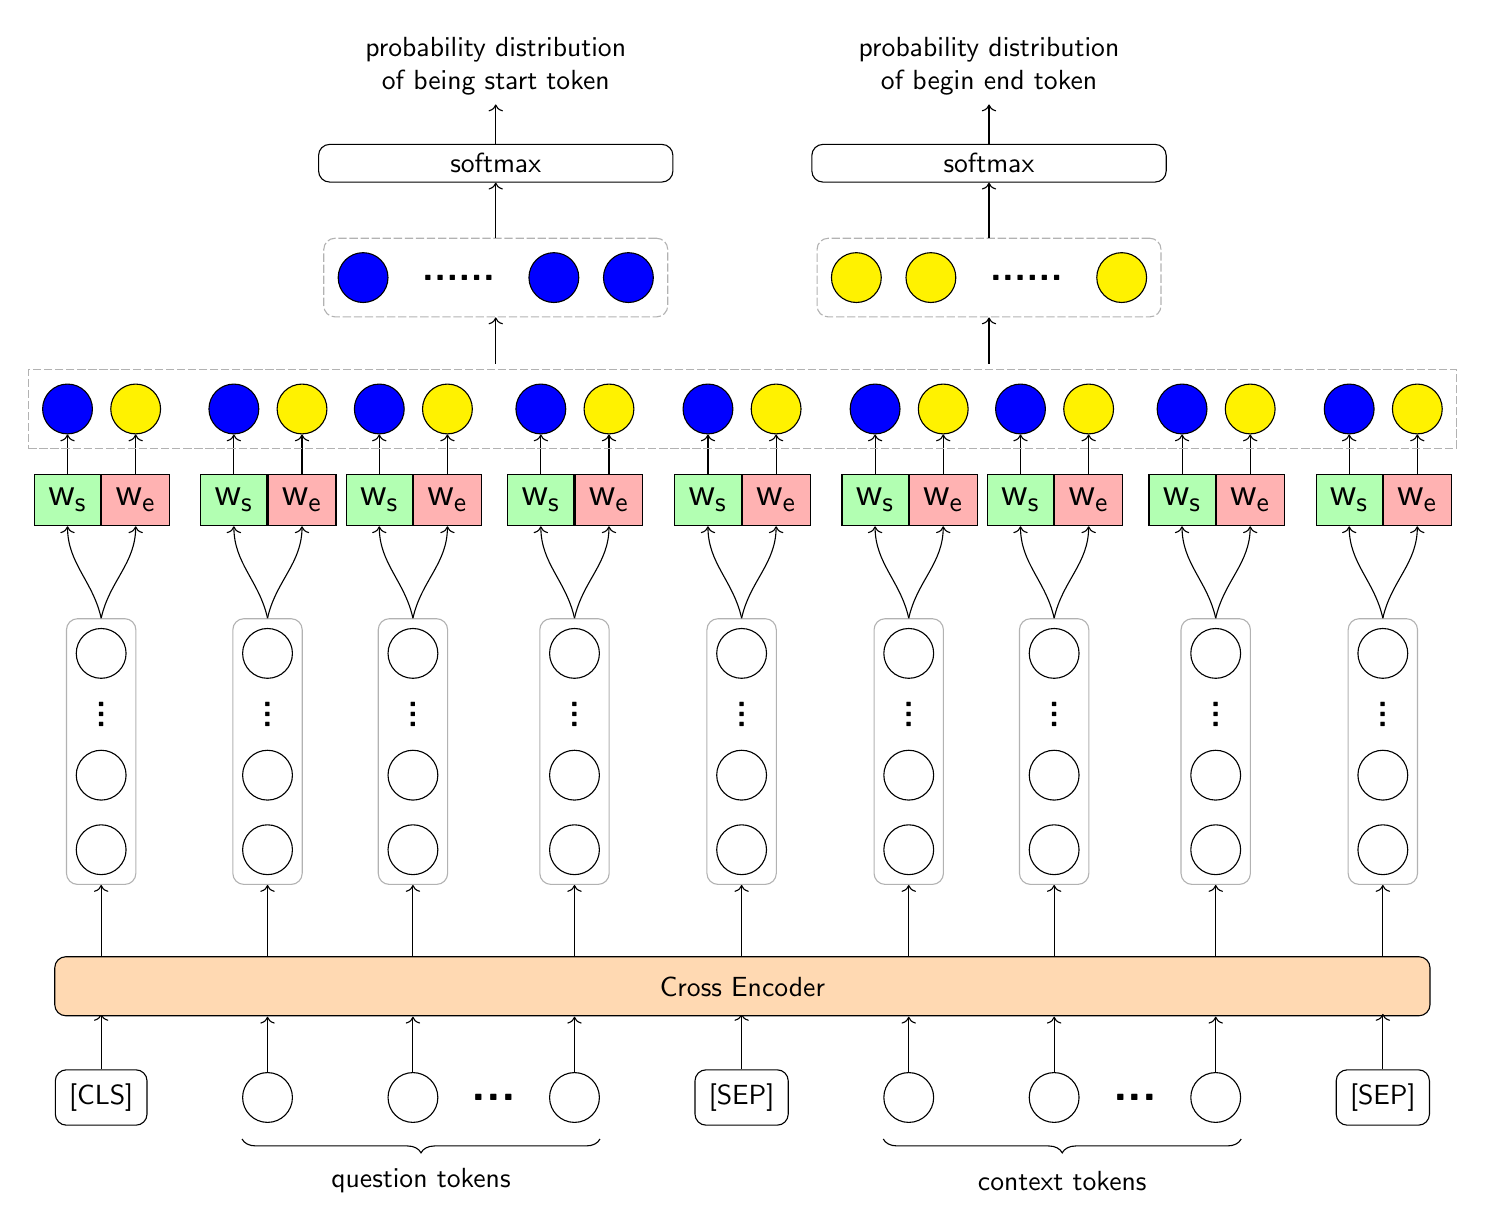
\begin{tikzpicture}[every node/.style={font=\sffamily}, align=center]
		\node [rounded corners, inner sep=5pt, draw=black] (qCLS) {[CLS]};
		\node [circle, draw=black, minimum size=18pt, right=1.2cm of qCLS] (qTok1) {};
		\node [circle, draw=black, minimum size=18pt, right=1.2cm of qTok1] (qTok2) {};
		\node [right=.3cm of qTok2, font=\fontsize{18pt}{\baselineskip}\selectfont\sffamily\bfseries] (qTokDots) {...};
		\node [circle, draw=black, minimum size=18pt, right=.3cm of qTokDots] (qTokLast) {};
		\node [rounded corners, draw=black, inner sep=5pt, minimum size=18pt, right=1.2cm of qTokLast] (qSEP) {[SEP]};
		\draw[->] (qCLS.north) -- ++ (0., 20pt);
		\draw[->] (qTok1.north) -- ++ (0., 20pt);
		\draw[->] (qTok2.north) -- ++ (0., 20pt);
		\draw[->] (qTokLast.north) -- ++ (0., 20pt);
		\draw[->] (qSEP.north) -- ++ (0., 20pt);
		\coordinate[yshift=-15pt] (braceAnchorLeft) at (qTok1.west);
		\coordinate[yshift=-15pt] (braceAnchorRight) at (qTokLast.east); 
		\draw [decorate,decoration={brace,amplitude=5pt,mirror}] (braceAnchorLeft) -- (braceAnchorRight) node[midway, yshift=-15pt]{question tokens};
		%% Context Encoder
		\node [circle, draw=black, minimum size=18pt, right=1.2cm of qSEP] (dTok1) {};
		\node [circle, draw=black, minimum size=18pt, right=1.2cm of dTok1] (dTok2) {};
		\node [right=.3cm of dTok2, font=\fontsize{18pt}{\baselineskip}\selectfont\sffamily\bfseries] (dTokDots) {...};
		\node [circle, draw=black, minimum size=18pt, right=.3cm of dTokDots] (dTokLast) {};
		\node [rounded corners, draw=black, inner sep=5pt, minimum size=18pt, right=1.2cm of dTokLast] (dSEP) {[SEP]};
		\coordinate[yshift=-15pt] (DbraceAnchorLeft) at (dTok1.west);
		\coordinate[yshift=-15pt] (DbraceAnchorRight) at (dTokLast.east); 
		\draw [decorate,decoration={brace,amplitude=5pt,mirror}] (DbraceAnchorLeft) -- (DbraceAnchorRight) node[midway, yshift=-15pt]{context tokens};
		%% Cross encoder
		\path let
		\p1 = (qCLS.west),
		\p2 = (qCLS.north)
		in
		coordinate (qCLSAnchor) at (\x1, \y2);
		\path let
		\p1 = (dSEP.east),
		\p2 = (dSEP.north)
		in
		coordinate (dSEPAnchor) at (\x1, \y2);
		\coordinate[shift={(0., 20.pt)}] (qEncLL) at (qCLSAnchor);
		\coordinate[shift={(0., 40.pt)}] (dEncUR) at (dSEPAnchor);
		\node (enc) [fit={(qEncLL) (dEncUR)}, inner sep=0pt, draw=black, text height=0.5cm, text depth=0.25cm, fill=orange!30, rounded corners] {Cross Encoder};
		\draw[->] (dTok1.north) -- ++ (0, 20pt);
		\draw[->] (dTok2.north) -- ++ (0, 20pt);
		\draw[->] (dTokLast.north) -- ++ (0, 20pt);
		\draw[->] (dSEP.north) -- ++ (0, 20pt);
		%==================================================================
		\node [circle, draw=black, minimum size=18pt, above=2.5cm of qTok1] (q2Tok1) {};
		\node [circle, draw=black, minimum size=18pt, above=2.5cm of qTok2] (q2Tok2) {};
		\node [circle, draw=black, minimum size=18pt, above=2.5cm of dTok1] (d2Tok1) {};
		\node [circle, draw=black, minimum size=18pt, above=2.5cm of dTok2] (d2Tok2) {};
		\node [circle, draw=black, minimum size=18pt, above=2.5cm of qTokLast] (qTokLast2) {};
		\node [circle, draw=black, minimum size=18pt, above=2.5cm of dTokLast] (dTokLast2) {};
		\path let
			\p1 = (q2Tok1.west),
			\p2 = (qCLS.north)
		in 
			coordinate (leftAnchor) at (\x2, \y1);
		\node [circle, draw=black, minimum size=18pt] (leftToken) at (leftAnchor) {};
		\path let
			\p1 = (dTokLast2.east),
			\p2 = (dSEP.north)
		in 
			coordinate (rightAnchor) at (\x2, \y1);
		\node [circle, draw=black, minimum size=18pt] (rightToken) at (rightAnchor) {};
		\path let
			\p1 = (qSEP.north),
			\p2 = (q2Tok1.east)
		in
			coordinate (midTokenAnchor) at (\x1, \y2);
		\node (midToken) [circle, draw=black, minimum size=18pt] at (midTokenAnchor) {};
		% ==========================================================
		\node (leftToken3) [above=0.3cm of leftToken, circle, draw=black, minimum size=18pt] {};
		\node (q3Tok1) [above=0.3cm of q2Tok1, circle, draw=black, minimum size=18pt] {};
		\node (q3Tok2) [above=0.3cm of q2Tok2, circle, draw=black, minimum size=18pt] {};
		\node (qTokLast3) [above=0.3cm of qTokLast2, circle, draw=black, minimum size=18pt] {};
		\node (midToken3) [above=0.3cm of midToken, circle, draw=black, minimum size=18pt] {};
		\node (d3Tok1) [above=0.3cm of d2Tok1, circle, draw=black, minimum size=18pt] {};
		\node (d3Tok2) [above=0.3cm of d2Tok2, circle, draw=black, minimum size=18pt] {};
		\node (dTokLast3) [above=0.3cm of dTokLast2, circle, draw=black, minimum size=18pt] {};
		\node (rightToken3) [above=0.3cm of rightToken, circle, draw=black, minimum size=18pt] {};
		% ==========================================================
		\node (leftToken4) [above=0.9cm of leftToken3, circle, draw=black, minimum size=18pt] {};
		\node (q4Tok1) [above=0.9cm of q3Tok1, circle, draw=black, minimum size=18pt] {};
		\node (q4Tok2) [above=0.9cm of q3Tok2, circle, draw=black, minimum size=18pt] {};
		\node (qTokLast4) [above=0.9cm of qTokLast3, circle, draw=black, minimum size=18pt] {};
		\node (midToken4) [above=0.9cm of midToken3, circle, draw=black, minimum size=18pt] {};
		\node (d4Tok1) [above=0.9cm of d3Tok1, circle, draw=black, minimum size=18pt] {};
		\node (d4Tok2) [above=0.9cm of d3Tok2, circle, draw=black, minimum size=18pt] {};
		\node (dTokLast4) [above=0.9cm of dTokLast3, circle, draw=black, minimum size=18pt] {};
		\node (rightToken4) [above=0.9cm of rightToken3, circle, draw=black, minimum size=18pt] {};
		% ==========================================================
		\path let
			\p1 = (leftToken3.north),
			\p2 = (leftToken4.south)
		in
			coordinate (leftTokenDots) at (\x1, \y1 / 2 + \y2 / 2);
		\node (leftTokenDotsText) [font=\fontsize{12pt}{\baselineskip}\selectfont\sffamily\bfseries, rotate=90] at (leftTokenDots) {...};
		\path let
			\p1 = (q3Tok1.north),
			\p2 = (q4Tok1.south)
		in
			coordinate (qDotsTok1) at (\x1, \y1 / 2 + \y2 / 2);
		\node (qDotsTok1Text) [font=\fontsize{12pt}{\baselineskip}\selectfont\sffamily\bfseries, rotate=90] at (qDotsTok1) {...};
		\path let
			\p1 = (q3Tok2.north),
			\p2 = (q4Tok2.south)
		in
			coordinate (qDotsTok2) at (\x1, \y1 / 2 + \y2 / 2);
		\node (qDotsTok2Text) [font=\fontsize{12pt}{\baselineskip}\selectfont\sffamily\bfseries, rotate=90] at (qDotsTok2) {...};
		\path let
			\p1 = (qTokLast3.north),
			\p2 = (qTokLast4.south)
		in
			coordinate (qTokenLastDots) at (\x1, \y1 / 2 + \y2 / 2);
		\node (qTokenLastDotsText) [font=\fontsize{12pt}{\baselineskip}\selectfont\sffamily\bfseries, rotate=90] at (qTokenLastDots) {...};
		\path let
			\p1 = (midToken3.north),
			\p2 = (midToken4.south)
		in 
			coordinate (midTokenDots) at (\x1, \y1 / 2 + \y2 / 2);
		\node (midTokenDotsText) [font=\fontsize{12pt}{\baselineskip}\selectfont\sffamily\bfseries, rotate=90] at (midTokenDots) {...};
		\path let
			\p1 = (d3Tok1.north),
			\p2 = (d4Tok1.south)
		in	
			coordinate (dDotsTok1) at (\x1, \y1 / 2 + \y2 / 2);
		\node (dDotsTok1Text) [font=\fontsize{12pt}{\baselineskip}\selectfont\sffamily\bfseries, rotate=90] at (dDotsTok1) {...};
		\path let 
			\p1 = (d3Tok2.north),
			\p2 = (d4Tok2.south)
		in
			coordinate (dDotsTok2) at (\x1, \y1 / 2 + \y2 / 2);
		\node (dDotsTok2Text) [font=\fontsize{12pt}{\baselineskip}\selectfont\sffamily\bfseries, rotate=90] at (dDotsTok2) {...};
		\path let 
			\p1 = (dTokLast3.north),
			\p2 = (dTokLast4.south)
		in
			coordinate (dTokLastDots) at (\x1, \y1 / 2 + \y2 / 2);
		\node (dTokLastDotsText) [font=\fontsize{12pt}{\baselineskip}\selectfont\sffamily\bfseries, rotate=90] at (dTokLastDots) {...};
		\path let 
			\p1 = (rightToken3.north),
			\p2 = (rightToken4.south)
		in
			coordinate (rightTokenDots) at (\x1, \y1 / 2 + \y2 / 2);
		\node (rightTokenDotsText) [font=\fontsize{12pt}{\baselineskip}\selectfont\sffamily\bfseries, rotate=90] at (rightTokenDots) {...};
		%========================================================
		\node (leftTokenBound) [fit={(leftToken4) (leftToken)}, draw=black!30, rounded corners] {};
		\node (qTok1Bound) [fit={(q4Tok1) (q2Tok1)}, draw=black!30, rounded corners] {};
		\node (qTok2Bound) [fit={(q4Tok2) (q2Tok2)}, draw=black!30, rounded corners] {};
		\node (qTokLastBound) [fit={(qTokLast4) (qTokLast2)}, draw=black!30, rounded corners] {};
		\node (midTokenBound) [fit={(midToken4) (midToken)}, draw=black!30, rounded corners] {};
		\node (dTok1Bound) [fit={(d4Tok1) (d2Tok1)}, draw=black!30, rounded corners] {};
		\node (dTok2Bound) [fit={(d4Tok2) (d2Tok2)}, draw=black!30, rounded corners] {};
		\node (dTokLastBound) [fit={(dTokLast4) (dTokLast2)}, draw=black!30, rounded corners] {};
		\node (rightTokenBound) [fit={(rightToken4) (rightToken)}, draw=black!30, rounded corners] {};
		% =========================================================
		\draw[<-] (leftTokenBound.south) -- ++ (0, -26pt);
		\draw[<-] (qTok1Bound.south) -- ++ (0, -26pt);
		\draw[<-] (qTok2Bound.south) -- ++ (0, -26pt);
		\draw[<-] (qTokLastBound.south) -- ++ (0, -26pt);
		\draw[<-] (midTokenBound.south) -- ++ (0, -26pt);
		\draw[<-] (dTok1Bound.south) -- ++ (0, -26pt);
		\draw[<-] (dTok2Bound.south) -- ++ (0, -26pt);
		\draw[<-] (dTokLastBound.south) -- ++ (0, -26pt);
		\draw[<-] (rightTokenBound.south) -- ++ (0, -26pt);
		% ==========================================================
		\coordinate[yshift=1.5cm] (anchorLeftTok) at (leftTokenBound.north) {}; 
		\node (greenMatLeft) [draw=black, inner sep=5pt, fill=green!30, left=0cm of anchorLeftTok, font=\fontsize{14pt}{\baselineskip}\selectfont\sffamily\bfseries] {$\mathsf{w_s}$};
		\node (redMatLeft) [draw=black, inner sep=5pt, fill=red!30, right=0cm of anchorLeftTok, font=\fontsize{14pt}{\baselineskip}\selectfont\sffamily\bfseries] {$\mathsf{w_e}$};
		\draw[->] (leftTokenBound.north)[xshift=-3pt] to[in=-90, out=90] (greenMatLeft.south);
		\draw[->] (leftTokenBound.north)[xshift=3pt] to[in=-90, out=90] (redMatLeft.south);
		\node (greenMatLeftAbove) [above=.5cm of greenMatLeft, circle, draw=black, minimum size=18pt, fill=blue] {};
		\node (redMatLeftAbove) [above=.5cm of redMatLeft, circle, draw=black, minimum size=18pt, fill=yellow] {};
		\draw[->] (greenMatLeft) -- (greenMatLeftAbove);
		\draw[->] (redMatLeft) -- (redMatLeftAbove);
		% ==========================================================
		\coordinate[yshift=1.5cm] (q2Anchor) at (qTok2Bound.north) {}; 
		\node (greenMatq2Anchor) [draw=black, inner sep=5pt, fill=green!30, left=0cm of q2Anchor, font=\fontsize{14pt}{\baselineskip}\selectfont\sffamily\bfseries] {$\mathsf{w_s}$};
		\node (redMatq2Anchor) [draw=black, inner sep=5pt, fill=red!30, right=0cm of q2Anchor, font=\fontsize{14pt}{\baselineskip}\selectfont\sffamily\bfseries] {$\mathsf{w_e}$};
		\draw[->] (qTok2Bound.north)[xshift=-3pt] to[in=-90, out=90] (greenMatq2Anchor.south);
		\draw[->] (qTok2Bound.north)[xshift=3pt] to[in=-90, out=90] (redMatq2Anchor.south);
		\node (greenMatq2AnchorAbove) [above=.5cm of greenMatq2Anchor, circle, draw=black, minimum size=18pt, fill=blue] {};
		\node (redMatq2AnchorAbove) [above=.5cm of redMatq2Anchor, circle, draw=black, minimum size=18pt, fill=yellow] {};
		\draw[->] (greenMatq2Anchor) -- (greenMatq2AnchorAbove);
		\draw[->] (redMatq2Anchor) -- (redMatq2AnchorAbove);
		% ==========================================================
		\coordinate[yshift=1.5cm] (q1Anchor) at (qTok1Bound.north) {}; 
		\node (greenMatq1Anchor) [draw=black, inner sep=5pt, fill=green!30, left=0cm of q1Anchor, font=\fontsize{14pt}{\baselineskip}\selectfont\sffamily\bfseries] {$\mathsf{w_s}$};
		\node (redMatq1Anchor) [draw=black, inner sep=5pt, fill=red!30, right=0cm of q1Anchor, font=\fontsize{14pt}{\baselineskip}\selectfont\sffamily\bfseries] {$\mathsf{w_e}$};
		\draw[->] (qTok1Bound.north)[xshift=-3pt] to[in=-90, out=90] (greenMatq1Anchor.south);
		\draw[->] (qTok1Bound.north)[xshift=3pt] to[in=-90, out=90] (redMatq1Anchor.south);
		\node (greenMatq1AnchorAbove) [above=.5cm of greenMatq1Anchor, circle, draw=black, minimum size=18pt, fill=blue] {};
		\node (redMatq1AnchorAbove) [above=.5cm of redMatq1Anchor, circle, draw=black, minimum size=18pt, fill=yellow] {};
		\draw[->] (greenMatq1Anchor) -- (greenMatq1AnchorAbove);
		\draw[->] (redMatq1Anchor) -- (redMatq1AnchorAbove);
		% ==========================================================
		\coordinate[yshift=1.5cm] (qTokLastAnchor) at (qTokLastBound.north) {}; 
		\node (matGreenQTokLast) [draw=black, inner sep=5pt, fill=green!30, left=0cm of qTokLastAnchor, font=\fontsize{14pt}{\baselineskip}\selectfont\sffamily\bfseries] {$\mathsf{w_s}$};
		\node (matRedQTokLast) [draw=black, inner sep=5pt, fill=red!30, right=0cm of qTokLastAnchor, font=\fontsize{14pt}{\baselineskip}\selectfont\sffamily\bfseries] {$\mathsf{w_e}$};
		\draw[->] (qTokLastBound.north)[xshift=-3pt] to[in=-90, out=90] (matGreenQTokLast.south);
		\draw[->] (qTokLastBound.north)[xshift=3pt] to[in=-90, out=90] (matRedQTokLast.south);
		\node (matGreenQTokLastAbove) [above=.5cm of matGreenQTokLast, circle, draw=black, minimum size=18pt, fill=blue] {};
		\node (matRedQTokLastAbove) [above=.5cm of matRedQTokLast, circle, draw=black, minimum size=18pt, fill=yellow] {};
		\draw[->] (matGreenQTokLast) -- (matGreenQTokLastAbove);
		\draw[->] (matRedQTokLast) -- (matRedQTokLastAbove);
		% ==========================================================
		\coordinate[yshift=1.5cm] (midTokenAnchor) at (midTokenBound.north) {}; 
		\node (greenMatMidToken) [draw=black, inner sep=5pt, fill=green!30, left=0cm of midTokenAnchor, font=\fontsize{14pt}{\baselineskip}\selectfont\sffamily\bfseries] {$\mathsf{w_s}$};
		\node (redMatMidToken) [draw=black, inner sep=5pt, fill=red!30, right=0cm of midTokenAnchor, font=\fontsize{14pt}{\baselineskip}\selectfont\sffamily\bfseries] {$\mathsf{w_e}$};
		\draw[->] (midTokenBound.north)[xshift=-3pt] to[in=-90, out=90] (greenMatMidToken.south);
		\draw[->] (midTokenBound.north)[xshift=3pt] to[in=-90, out=90] (redMatMidToken.south);
		\node (greenMatMidTokenAbove) [above=.5cm of greenMatMidToken, circle, draw=black, minimum size=18pt, fill=blue] {};
		\node (redMatMidTokenAbove) [above=.5cm of redMatMidToken, circle, draw=black, minimum size=18pt, fill=yellow] {};
		\draw[->] (greenMatMidToken) -- (greenMatMidTokenAbove);
		\draw[->] (redMatMidToken) -- (redMatMidTokenAbove);
		% ==========================================================
		\coordinate[yshift=1.5cm] (dTok1Anchor) at (dTok1Bound.north) {}; 
		\node (greenMatTok1) [draw=black, inner sep=5pt, fill=green!30, left=0cm of dTok1Anchor, font=\fontsize{14pt}{\baselineskip}\selectfont\sffamily\bfseries] {$\mathsf{w_s}$};
		\node (redMatTok1) [draw=black, inner sep=5pt, fill=red!30, right=0cm of dTok1Anchor, font=\fontsize{14pt}{\baselineskip}\selectfont\sffamily\bfseries] {$\mathsf{w_e}$};
		\draw[->] (dTok1Bound.north)[xshift=-3pt] to[in=-90, out=90] (greenMatTok1.south);
		\draw[->] (dTok1Bound.north)[xshift=3pt] to[in=-90, out=90] (redMatTok1.south);
		\node (greenMatTok1Above) [above=.5cm of greenMatTok1, circle, draw=black, minimum size=18pt, fill=blue] {};
		\node (redMatTok1Above) [above=.5cm of redMatTok1, circle, draw=black, minimum size=18pt, fill=yellow] {};
		\draw[->] (greenMatTok1) -- (greenMatTok1Above);
		\draw[->] (redMatTok1) -- (redMatTok1Above);
		% ==========================================================
		\coordinate[yshift=1.5cm] (dTok2Anchor) at (dTok2Bound.north) {}; 
		\node (greenMatdTok2) [draw=black, inner sep=5pt, fill=green!30, left=0cm of dTok2Anchor, font=\fontsize{14pt}{\baselineskip}\selectfont\sffamily\bfseries] {$\mathsf{w_s}$};
		\node (redMatdTok2) [draw=black, inner sep=5pt, fill=red!30, right=0cm of dTok2Anchor, font=\fontsize{14pt}{\baselineskip}\selectfont\sffamily\bfseries] {$\mathsf{w_e}$};
		\draw[->] (dTok2Bound.north)[xshift=-3pt] to[in=-90, out=90] (greenMatdTok2.south);
		\draw[->] (dTok2Bound.north)[xshift=3pt] to[in=-90, out=90] (redMatdTok2.south);
		\node (greenMatdTok2Above) [above=.5cm of greenMatdTok2, circle, draw=black, minimum size=18pt, fill=blue] {};
		\node (redMatdTok2Above) [above=.5cm of redMatdTok2, circle, draw=black, minimum size=18pt, fill=yellow] {};
		\draw[->] (greenMatdTok2) -- (greenMatdTok2Above);
		\draw[->] (redMatdTok2) -- (redMatdTok2Above);
		% ==========================================================
		\coordinate[yshift=1.5cm] (dTokLastAnchor) at (dTokLastBound.north) {}; 
		\node (greenMatDTokLast) [draw=black, inner sep=5pt, fill=green!30, left=0cm of dTokLastAnchor, font=\fontsize{14pt}{\baselineskip}\selectfont\sffamily\bfseries] {$\mathsf{w_s}$};
		\node (redMatDTokLast) [draw=black, inner sep=5pt, fill=red!30, right=0cm of dTokLastAnchor, font=\fontsize{14pt}{\baselineskip}\selectfont\sffamily\bfseries] {$\mathsf{w_e}$};
		\draw[->] (dTokLastBound.north)[xshift=-3pt] to[in=-90, out=90] (greenMatDTokLast.south);
		\draw[->] (dTokLastBound.north)[xshift=3pt] to[in=-90, out=90] (redMatDTokLast.south);
		\node (greenMatDTokLastAbove) [above=.5cm of greenMatDTokLast, circle, draw=black, minimum size=18pt, fill=blue] {};
		\node (redMatDTokLastAbove) [above=.5cm of redMatDTokLast, circle, draw=black, minimum size=18pt, fill=yellow] {};
		\draw[->] (greenMatDTokLast) -- (greenMatDTokLastAbove);
		\draw[->] (redMatDTokLast) -- (redMatDTokLastAbove);
		% ==========================================================
		\coordinate[yshift=1.5cm] (rightTokAnchor) at (rightTokenBound.north) {}; 
		\node (greenMatright) [draw=black, inner sep=5pt, fill=green!30, left=0cm of rightTokAnchor, font=\fontsize{14pt}{\baselineskip}\selectfont\sffamily\bfseries] {$\mathsf{w_s}$};
		\node (redMatright) [draw=black, inner sep=5pt, fill=red!30, right=0cm of rightTokAnchor, font=\fontsize{14pt}{\baselineskip}\selectfont\sffamily\bfseries] {$\mathsf{w_e}$};
		\draw[->] (rightTokenBound.north)[xshift=-3pt] to[in=-90, out=90] (greenMatright.south);
		\draw[->] (rightTokenBound.north)[xshift=3pt] to[in=-90, out=90] (redMatright.south);
		\node (greenMatrightAbove) [above=.5cm of greenMatright, circle, draw=black, minimum size=18pt, fill=blue] {};
		\node (redMatrightAbove) [above=.5cm of redMatright, circle, draw=black, minimum size=18pt, fill=yellow] {};
		\draw[->] (greenMatright) -- (greenMatrightAbove);
		\draw[->] (redMatright) -- (redMatrightAbove);
		% ==========================================================
		\node [draw=black!30, dash pattern=on 3pt off 1pt, inner sep=5pt, fit={(greenMatLeftAbove)(redMatrightAbove)}] {};
		% ==========================================================
		\node [yshift=9cm] (anchorCenter) at (enc) {};
		\node (leftMost) [circle, draw=black, fill=blue, minimum size=18pt, left=1.cm of anchorCenter] {};
		\node (leftMost2) [circle, draw=black, fill=blue, minimum size=18pt, left=.3cm of leftMost] {};
		\node (leftMostDots) [left=.3cm of leftMost2, font=\fontsize{14pt}{\baselineskip}\selectfont\sffamily\bfseries] {......};
		\node (leftMost3) [circle, draw=black, fill=blue, minimum size=18pt, left=.3cm of leftMostDots] {};
		\node [inner sep=5pt, rounded corners, dash pattern=on 3pt off 1pt, draw=black!30, fit={(leftMost) (leftMost3)}] (boundLeft) {};
		% ==========================================================
		\node (rightMost) [circle, draw=black, fill=yellow, minimum size=18pt, right=1.cm of anchorCenter] {};
		\node (rightMost2) [circle, draw=black, fill=yellow, minimum size=18pt, right=.3cm of rightMost] {};
		\node (rightMostDots) [right=.3cm of rightMost2, font=\fontsize{14pt}{\baselineskip}\selectfont\sffamily\bfseries] {......};
		\node (rightMost3) [circle, draw=black, fill=yellow, minimum size=18pt, right=.3cm of rightMostDots] {};
		\node [inner sep=5pt, rounded corners, dash pattern=on 3pt off 1pt, draw=black!30, fit={(rightMost) (rightMost3)}] (boundRight) {};
		% ==========================================================
		\draw [<-] (boundLeft.south) -- ++ (0, -17pt);
		\draw [<-] (boundRight.south) -- ++ (0, -17pt);
		% ----------------------------------------------------------
		\node (softmaxLeft) [above=.7cm of boundLeft, draw=black, rounded corners, minimum width=4.5cm] {softmax};
		\node (softmaxRight) [above=.7cm of boundRight, draw=black, rounded corners, minimum width=4.5cm] {softmax};
		\draw[->] (boundLeft) -- (softmaxLeft);
		\draw[->] (boundRight) -- (softmaxRight);
		\node (finalLeft) [above=0.5cm of softmaxLeft] {probability distribution \\of being start token};
		\node (finalRight) [above=0.5cm of softmaxRight] {probability distribution \\of begin end token};
		\draw[->] (softmaxLeft) -- (finalLeft);
		\draw[->] (softmaxRight) -- (finalRight);
	\end{tikzpicture}
\end{document}